%!TEX root = ../report.tex

\todo{Purpose of the chapter
 Structure of the chapter
 Central themes of the chapter}

\section{Non-functional requirements} {
\label{sec:non_functiona_requirements}

	The following non-functional requirements are considered key to the success of this project:

	\begin{description}
		\item[Modularity:] The project should be highly modular, so parts of the system can be reused and easily integrated into the group project.
		\item[Performance:] The response time of the system is a major concern when working with a large dataset. The time to load the visualisation is highly dependent on the size of the dataset, graphical processing, network bandwidth and latency. However, once the visualisation has loaded, the user should be faced with near immediate response times (\textless 1 second).
		\item[Scalability:] This is important when modifying the size of the dataset used with a visualisation. The visualisation should be capable of handling increased processing with a larger dataset. Not only this, but the information should remain mapped to the correct locations in the scene with increased volumes of data.
		\item[Testability:] Highly testable code is important when writing test suites, so all aspects of the system can be easily tested to locate faults. In JavaScript:
			\begin{itemize}
				\item A common technique is to hide variables through the use of closure, which leads to untestable code. These variables should be replaced with public variables that are prefixed with an underscore, to indicate they are not a part of the public API.
				\item Promises should not be used within a constructor.
				\item Anonymous functions should be replaced with named functions so they can be tested.
				\item Dependency injection should be used through RequireJS, so all dependencies can be mocked.
			\end{itemize}
	\end{description}

}

\section{Methodology} {
\label{sec:methodology}

	A rapid application development (RAD) approach was undertaken when developing this project. This methodology focuses on iterative development and the rapid construction of prototypes, instead of investing significant amounts of time into planning. RAD enables the software to be written quickly through the reuse of software components and engaging in less formal reviews. This process also performs unit, integration and system testing at the end of each construction phase.

	\todo{insert diagram}

	In this project, each visualisation can be thought of as a single prototype, where parts of the first prototype can be reused for the second visualisation. Testing should be performed during the course of the project, but particularly when a major component of a prototype has been developed, such as data filtering.

	\todo{iterative, agile}

	% An agile methodology will be used throughout the project, as it promotes iterative development, adaptive planning, early prototyping, and encourages flexible and rapid response to changing requirements. This is in contrast to the more traditional methodology, waterfall, which implies a much more rigid workflow, where all requirements are set in stone early in the project. The agile approach gives the project more flexibility, which is required for a project of greater complexity.
	
	% \subsection{Scrum} {

	% 	Scrum is an iterative and incremental agile methodology, in consists of short iterative `sprints' of focused development. The decided sprint length of this project 2 weeks, and conveniently corresponds with the fortnightly client meetings.
		
	% 	Before each sprint, tasks are created and prioritised. These tasks are then assigned evenly across team leaders, and then are further distributed to their team members. This process can take a day or so after the last sprint has finished, using the client's feedback as motivation as to what to include in the sprint. A sprint is then started, and development is generally 'locked' until the completion of the sprint. This keeps teams focused on the issues for the sprint, which have been decided to be the most important.
		
	% 	The chosen issue tracking tool, JIRA, wholly supports the scrum methodology, with in-built features for creating sprints, epics and user stories. This in-built tooling support, combined with its iterative development cycle, makes Scrum a convenient and appropriate methodology for the project.
		
}

\section{Dataset} {
\label{sec:dataset}

	As discussed in Section~\ref{sec:project_definition}, the visualisations began with generated data so development could begin immediately. Using generated data brings control over the size of the dataset applied to a prototype and enables the scalability of each visualisation can be tested. 

	\todo{convert rest of stuff from interim to past tense and make datasets solid}

	% Following the use of fake data, each prototype had real datasets applied to them. By using the same data for both prototypes, their differences in computational requirements and scalability could be compared and analysed. GeoNames~\footnote{\bibentry{wick2005geonames}} is a geographical database that stores population data for a significant number of cities and their respective latitude and longitude coordinates. This database falls under a creative commons attribution license and will be used for both visualisations because there are no copyright concerns or immediate issues when reading and parsing the data it provides. However, some unnecessary information contained in a GeoNames dataset (such as \emph{geonameid}, \emph{feature class} and  \emph{dem}) will need to be removed. The format of the data should also be modified (from a tab separated list to a JavaScript array) when used with a prototype. These steps are necessary so the visualisations can read the data efficiently and hence reduce the loading time for the user. Other datasets can be obtained from Earthdata~\footnote{\bibentry{nasa2000data}}, but will require further investigation regarding how to extract the information from the available databases.

	% Once real data has been applied to both prototypes, the visualisations will be integrated into a live system for the teaching analytics component of the final year project. The amount of touch gestures that particular system components receive and the progress made by students, groups and tutorials will need to be collected and stored in the database. This data can be visualised to aid teachers in analysing ongoing student progress.

	\subsection{Structure} {
	\label{sec:dataset_structure}

		\todo{mention flat vs metadata, performance issues}


	}

}

\section{User interface} {
\label{sec:user_interface}

	The graphical user interface (GUI) for this system has combined Google's Material Design with a 3D environment, to simplify the way users interact with the system.

	\subsection{Material Design} {
	\label{sec:material_design}

		Material Design is a visual language developed by Google that synthesises classic design principles with current technologies. Their design aims to provide users with a unified experience across platforms and device sizes, by focusing on user actions and retaining continuity between transitions~\footnote{\bibentry{google2015material}}. Furthermore, Material Design provides an immersive experience to users by adhering to good design principles.

		Google Material Design details many component specifications that have been implemented by several CSS3 frameworks. It is also a great design tool that has been incorporated into the existing infrastructure this project and the group project. As a result of this, a teacher can transition from one system to the other seamlessly, because both systems apply the same design standards.

	}

	\subsection{3D environment} {
	\label{sec:3d_environment}

		The visualisation being viewed by a user features a 3D environment. It has been designed with the following in mind:

		\begin{itemize}
			\item Navigation interactions -- pan, zoom and rotate.
			\item Data points that represent the dataset are displayed as either 3D bars or NURBS.
				\begin{itemize}
					\item Data points should have the ability to be filtered.
				\end{itemize}
			\item The colour of a data point should be effected by the value it represents.
				\begin{itemize}
					\item e.g. Data points that represent population data may be coloured red, orange or yellow to indicate high, medium or low population areas respectively.
				\end{itemize}
			\item Information associated with a data point can be viewed by a user.
				\begin{itemize}
					\item Should use a simple panel interface, shown in Figure~\ref{fig:information_display_design}.
					\item Information is retrieved through metadata. 
					\item Can be shown through hover effects or by outputting the dataset on the page.
				\end{itemize}
			\item Data points are projected from a base geometry.
				\begin{itemize}
					\item The geometry can be a plane or sphere and depends on the dataset being used.
				\end{itemize}
			\item A skybox should serve as a static background for the environment.
		\end{itemize}

		%!TEX root = ../../report.tex

\begin{figure}[H]
	\centering
	\newcommand{\figurewidth}{0.4\textwidth}
	\centering
	\begin{subfigure}[b]{\figurewidth}
        \figureborder{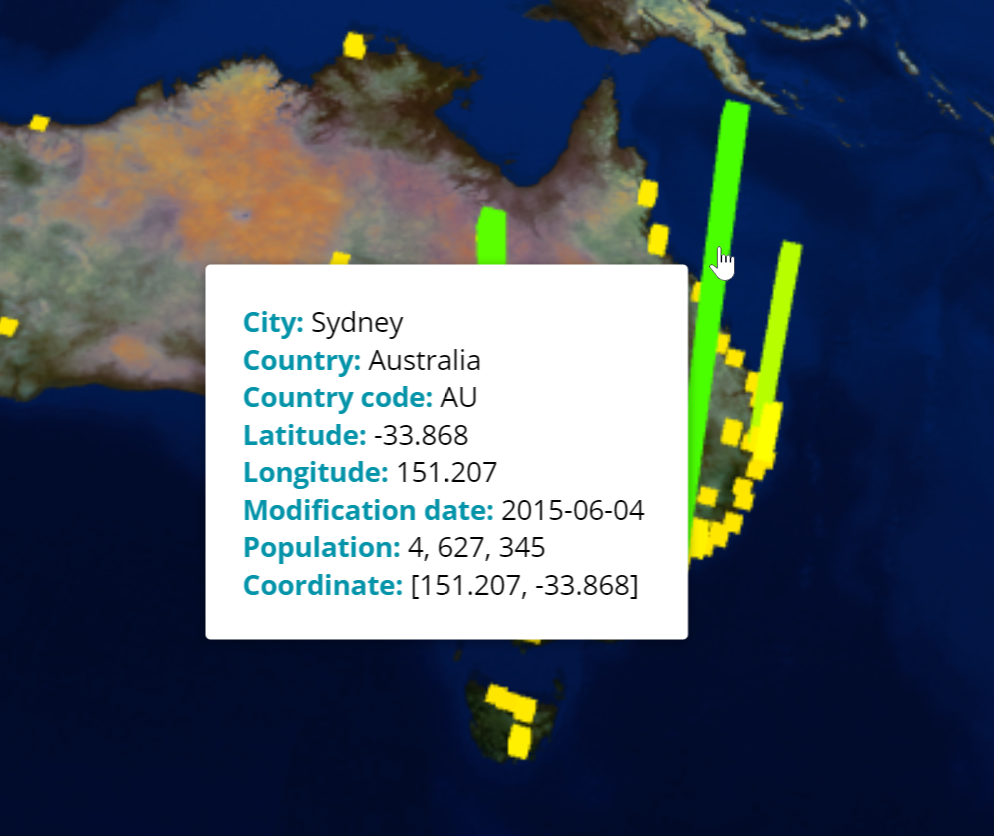
\includegraphics[width=\textwidth]{images/implementation/information_display/population}}
		\caption{Information display for population data.}
		\label{fig:information_display_population}
	\end{subfigure}
	\begin{subfigure}[b]{\figurewidth}
		\figureborder{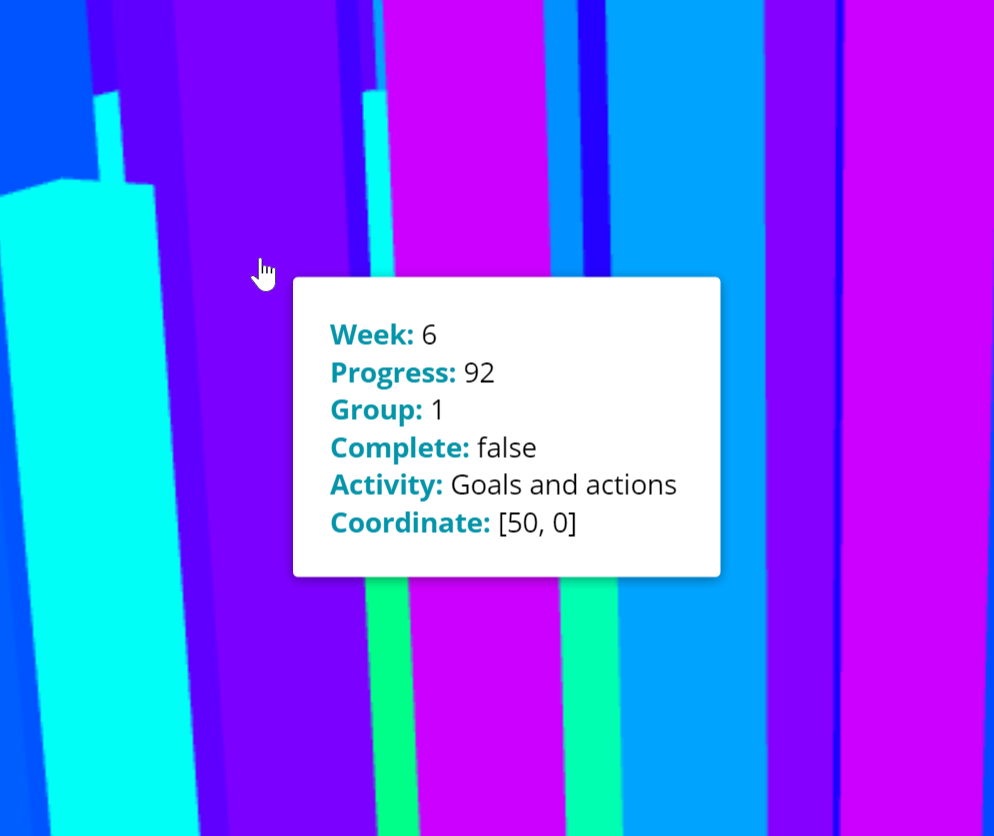
\includegraphics[width=\textwidth]{images/implementation/information_display/student}}
		\caption{Information display for student data.}
		\label{fig:information_display_student}
	\end{subfigure}
	\caption[Information display]{Information display hover effect.}
	\label{fig:information_display}
\end{figure}


		Example mockups of the 3D environment that fulfil the above criteria have been demonstrated in Figure~\ref{fig:environment_mockups}.

		%!TEX root = ../../../report.tex

\begin{figure}[H]
    \newcommand{\figurewidth}{0.5\textwidth}
    \newcommand{\figureheight}{3cm}
	\begin{subfigure}[b]{\figurewidth}
        \centering
        \raisebox{0.5\height}{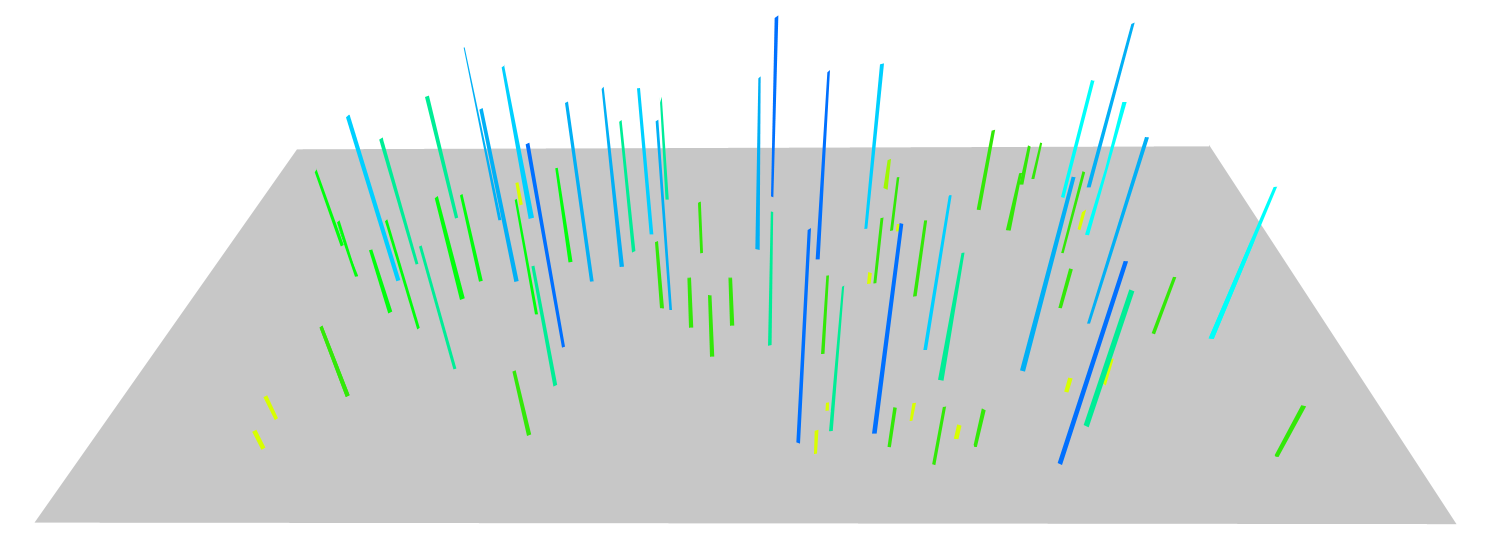
\includegraphics[width=\textwidth]{images/design/mockups/flat}}
        \caption{Visualisation using a flat surface.}
        \label{fig:visualisation_flat}
    \end{subfigure}
    \begin{subfigure}[b]{\figurewidth}
        \centering
        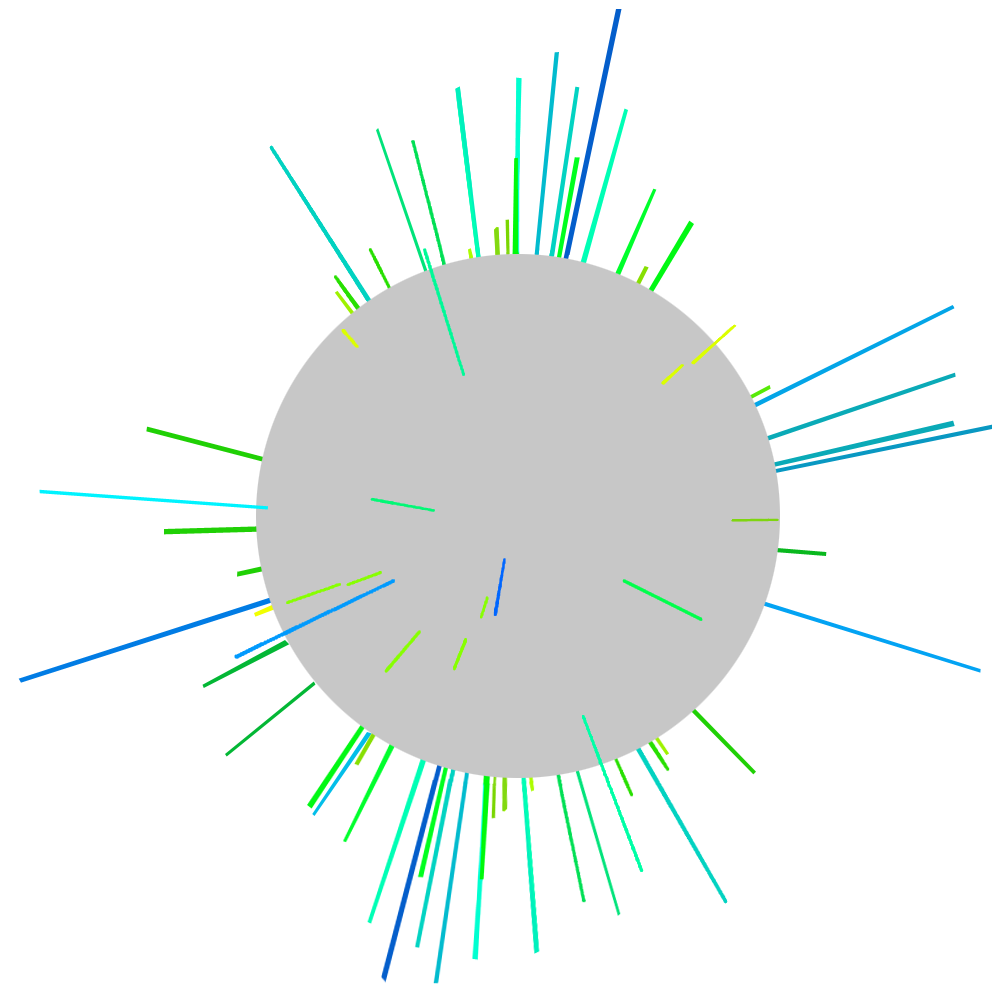
\includegraphics[width=\textwidth]{images/design/mockups/sphere}
        \caption{Visualisation using a sphere surface.}
        \label{fig:visualisation_sphere}
    \end{subfigure}
	\caption[3D environment mockups]{3D environment mockups.}
	\label{fig:environment_mockups}
\end{figure}


	}

	\subsection{Interface design} {
	\label{sec:interface_design}

		The design of the interface needs to account for both the use of Material Design and the 3D environment. 

		Material Design is renowned for its sliding drawer menu, often used to maximise the viewing space for the user. This component has the potential to maintain user focus on the visualisation, while providing additional information through an unobtrusive menu. An initial mockup of this design has been demonstrated in Figure~\ref{fig:user_interface_mockup}, where the 3D environment fills the content to the right of the drawer. This design has been refined through the implementation phase described in Section~\ref{sec:filtering_implementation} and \ref{sec:configuration_implementation}.

		%!TEX root = ../../../report.tex

\begin{figure}[H]
	\centering
    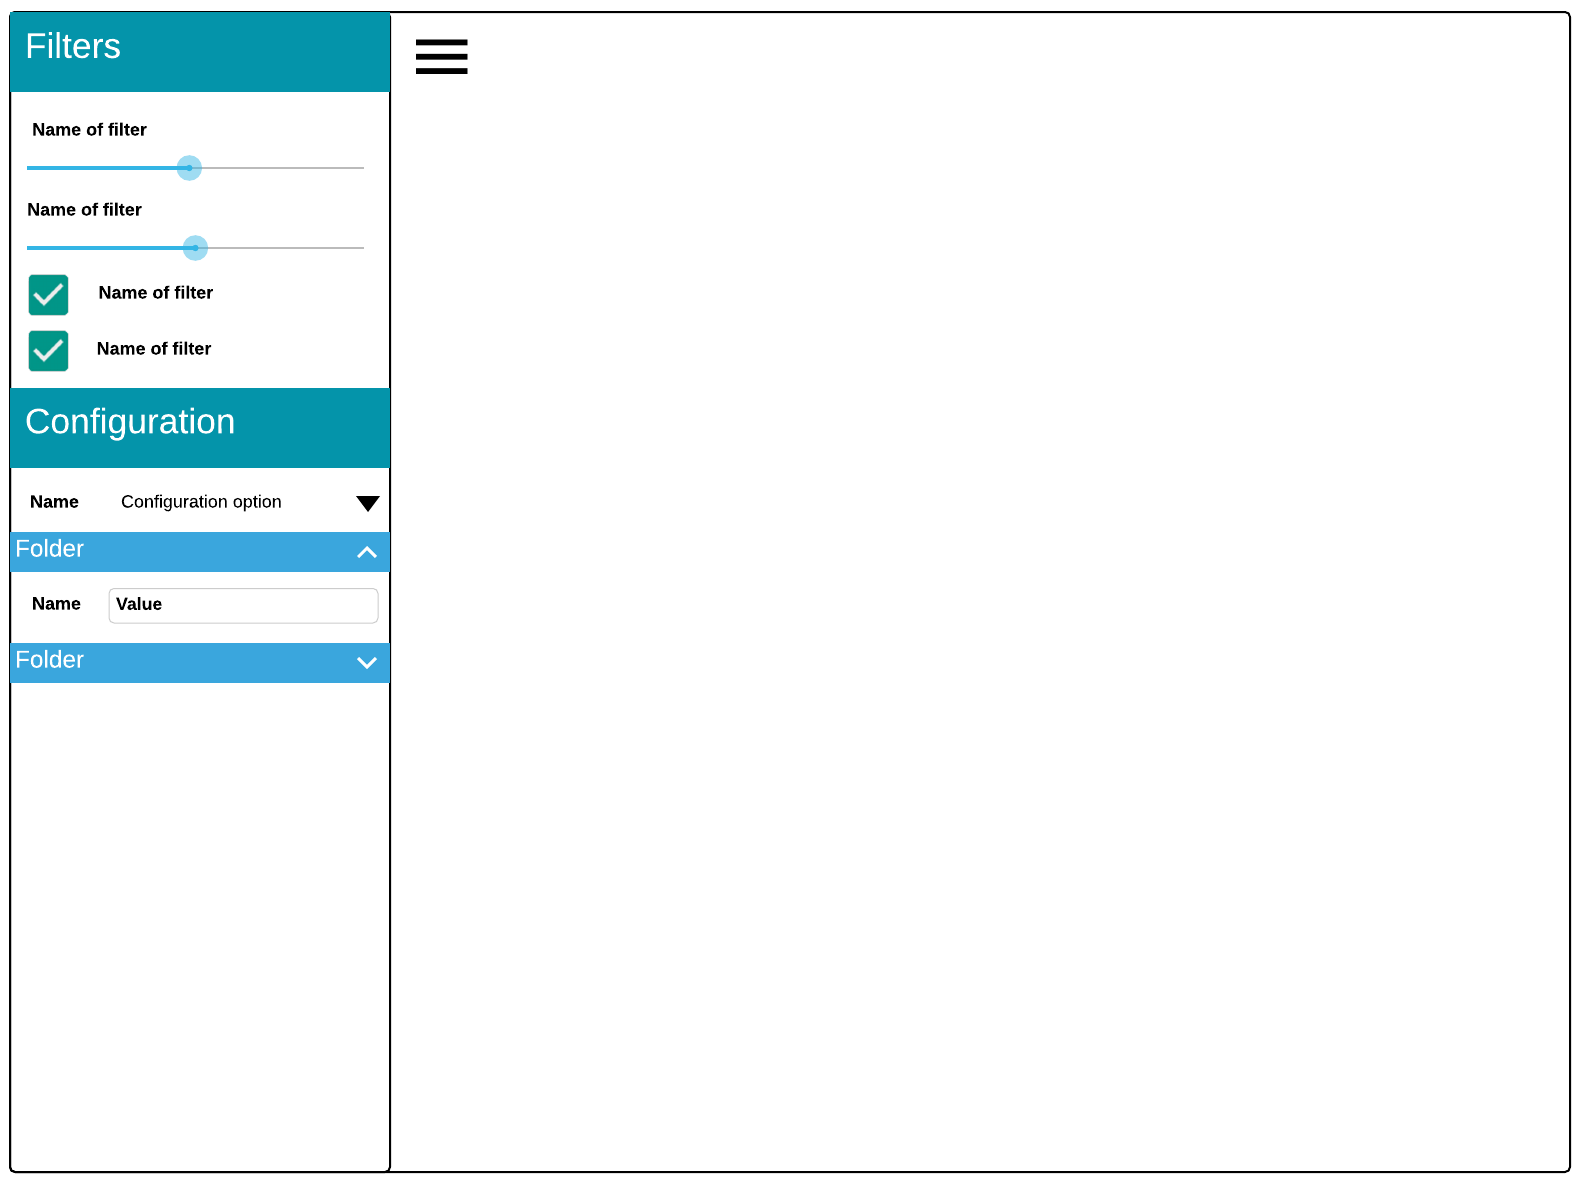
\includegraphics[width=\textwidth]{images/design/mockups/interface}
    \caption[User interface mockup]{User interface mockup.}
    \label{fig:user_interface_mockup}
\end{figure}


		The sliding drawer utilises Material Design components and incorporates two main features -- filtering and live configuration.

		\subsubsection{Filtering} {
		\label{sec:filtering}

			Filters take advantage of slider and checkbox widgets to adjust the state of what is displayed to the user.

			\emph{Sliders} adjust what data points are visible to the user. This is achieved by configuring the bounds of the available metadata in a data point. Take for example a dataset that has a range of values between 0 -- 100. If the user adjusts the value of its respective slider to be $\ge$20, then any data points that have a value \textless20 will be hidden.
			
			\emph{Checkboxes} are designed to be toggled on or off. This widget toggles what metadata associated with a data point is displayed to the user.

		}

		\subsubsection{Configuration} {
		\label{sec:configuration}

			Configuration options are designed to change the values and attributes of the 3D environment in real-time, promoting the analysis of the effects colour has on useability and performance. These options are organised in a folder structure, to deliver a hierarchy and logical grouping to the user. Moreover, these options should handle configuring data points and surface values which enable the user to customise the display of the system.

			\emph{Data point} configurations should modify the low, medium, high colour values and the range of colours displayed.

			\emph{Surface} configurations should modify the midtone colours of the surface and the colour or intensity of other surface attributes.

		}

	}

}

\section{User actions} {
\label{sec:user_actions}

	The interactions that a user can perform when using this system have been represented in Figure~\ref{fig:user_actions}.

	%!TEX root = ../../report.tex

\begin{figure}[H]
	\centering
    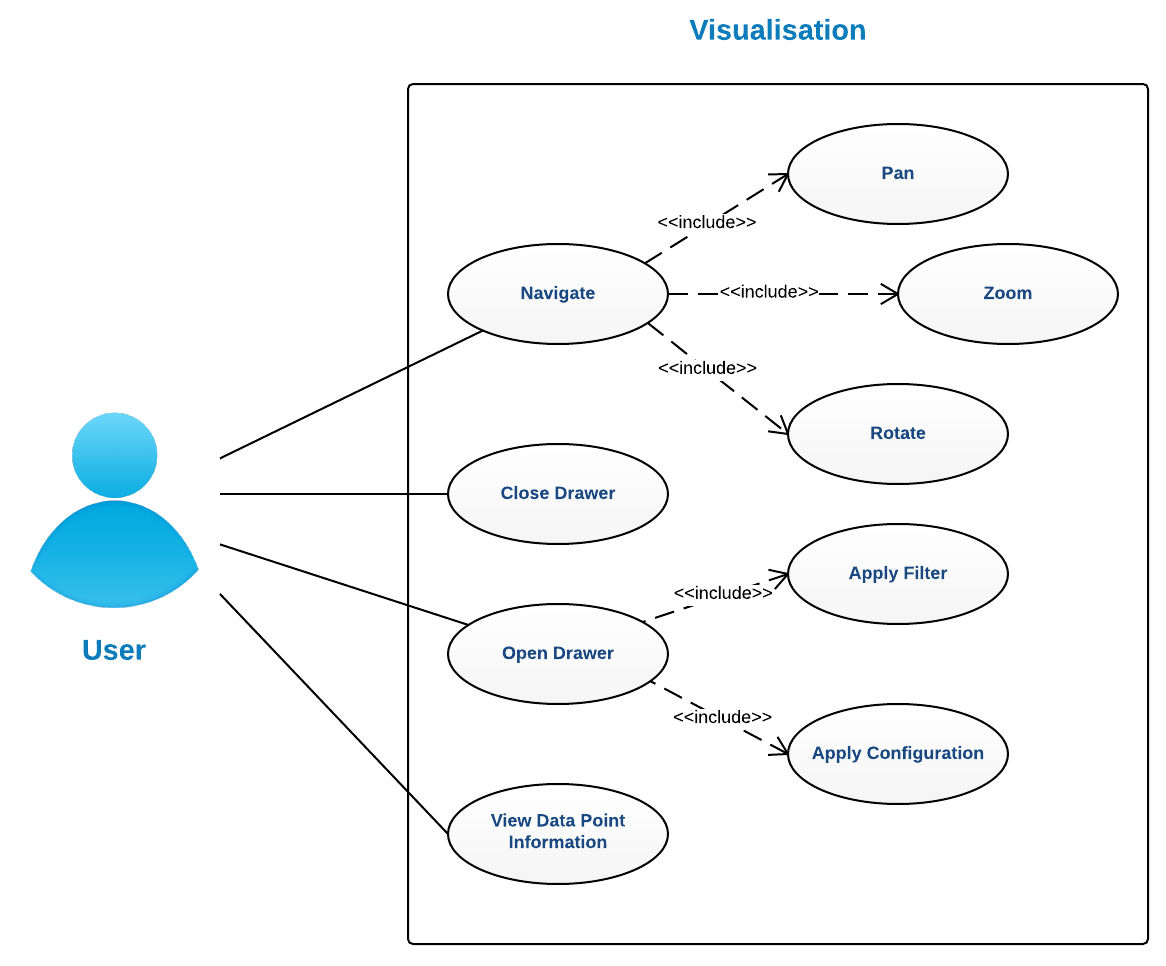
\includegraphics[height=10cm]{images/design/user_actions}
    \caption[User actions]{User actions use-case diagram.}
    \label{fig:user_actions}
\end{figure}


	These user actions facilitate decision making processes by allowing users to evaluate different datasets and identify key features. For instance, when the user navigates around the scene they are able to view the information associated with a data point by hovering on it. In regards to population data the smallest and largest city or country can be established using this method. This is achieved by navigating to a short or tall data point and displaying its information which contains details such as the city and country. Similarly, when a student dataset is used the best and worst performing groups can be identified on a weekly and on an average basis by analysing this information. Viewing student progress in such a manner can also aid in determining patterns with particular groups and individuals, and examining the overall complexity of a task during certain weeks. 

	When filtering is applied to any dataset, the user can quickly confirm their initial observations found during the navigate and view data point information actions. This is due to the fact that a filter can determine which data points are visible to the user, by adjusting the minimum and maximum range of a property in the dataset through a widget. As an example, displaying populations that are either below or over 100,~000 individuals can easily be seen by adjusting the minimum or maximum filter bounds for the population property to 100,~000.

	Finally, different configurations can be applied in order to customise the appearance of the environment. This is achieved so that a distinguished colour scheme for the data points and surface is selected. In turn, this can enhance a user's ability to identify significant features and patterns through colour palettes that make the dataset clearer to understand.

}

\section{Architecture} {
\label{sec:architecture}
	
	\todo{three-tier: presentation, logic, data

		inheritance

		design patterns

		forwards ajax request to backend of fyp system for dataset

		}

		\todo{Everything implemented as a single module, write more / reword}

		The Filter, Configuration, and Information display modules are external to the core 3D environment components, separating the components in the scene from the view controllers. This design decision also ensures that the view controllers can be removed from the application at any time, without effecting the core functionality.

		%!TEX root = ../../report.tex

\begin{figure}[H]
	\centering
    \includegraphics[width=\textwidth]{images/design/architecture}
    \caption[Architecture]{System architecture.}
    \label{fig:architecture}
\end{figure}


% 		The frontend system is a separate client-server application, consisting of a node.js server component, which simply pushes the Client-side component to the client-browser. The client-side therefore contains the vast majority of application complexity which has the following architecture:
% Uses a MVVM (Model View View-Model) architectural style to compose data bound from performing asynchronous requests to the backend API, with the view-templates via the View-Model (controllers).
% The API-Client 
% Much of the 'heavy lifting' of data manipulation is delegated to the backend API.
% View-templates are a set of DSL template files that compose a particular UI component
% These are dynamically compiled into views, incorporating data from the model.
% The primary function of the View-Model (depicted as controllers) is to bind changes to the Model data and update the Views accordingly.
% Conceptually this functionality requires a data-mapping sub-module, but it is likely that this will be provided by a library.
% This all occurs in an asynchronous Event-based manner, such that the UI is never blocked.


}

\section{Evaluations} {
\label{sec:evaluation_design}

	\todo{}

}
